\chapter{Systematic uncertainties on simulated samples}\label{chap:sysmc}

Due to the data-driven nature of the analysis, uncertainties related to the simulated samples are not directly applied since the simulated samples are only used to validate the data-driven background estimation. Instead, these uncertainties enter as a second order effect and are used to calculate the uncertainty associated with the data-driven background estimation. Uncertainties that exhibit normalisation changes have marginal impact on the data-driven background estimation. The largest impact arises from the systematic uncertainties which are related to changes in the shape of the invariant-mass distribution. This is discussed further in \cref{chap:bkgmodel}. The sources of systematic uncertainties on the simulated samples are outlined in this section. 

There are several systematic uncertainties that affect the background modelling of the simulated samples, and these uncertainties can be divided into two distinct categories: experimental uncertainties related to the event (e.g. luminosity measurement) and to the reconstruction of the physics objects described in \cref{chap:SimReco}, and uncertainties from theoretical predictions from the PDF. The experimental uncertainties are outlined in \cref{sec:sysmc:exp} and the theoretical uncertainties are outlined in \cref{sec:sysmc:theory}. The theoretical background uncertainty variations are estimated as a function of the true invariant-mass, where the transfer function approach, described in \cref{sec:datamc:transfer}, is applied to generate high-statistic and smooth reconstructed templates for the uncertainties. The experimental uncertainties are provided by dedicated groups in charge of the performance of electron and muon reconstruction.

\section{Experimental uncertainties}\label{sec:sysmc:exp}

\subsection{Event uncertainties}
Uncertainties on the luminosity and the pileup measurements affect the overall normalisation of the processes being studied. The measurement of the luminosity is described in \cref{sec:method:lumi} and the uncertainty is calculated using the method described in \cite{Aaboud:2208146}. For the full Run-2 dataset used in this analysis, the luminosity uncertainty is calculated to be $\pm 1.7\%$. The uncertainty on the pileup distributions is measured by taking the difference between the pileup distribution observed in data and those expected at the time of producing the MC simulations. Additionally, uncertainties on the efficiency of the triggers used in the analysis are also considered.  \cref{fig:uncert:prwuncert} depicts the effect of the pileup uncertainty on the invariant mass distribution for the electron and muon channels. The figure shows that contribution from the pileup reweighting uncertainty is less than 1\% for both the electron and the muon channels. This will result in a negligible impact on the background estimation. The difference in shape of the systematic variation between the electron and muon channel is due to statistical fluctuation in the muon channel that result in a less smooth distribution. 

\begin{figure}[h!]
    \centering
    \begin{subfigure}[h]{0.42\textwidth}
        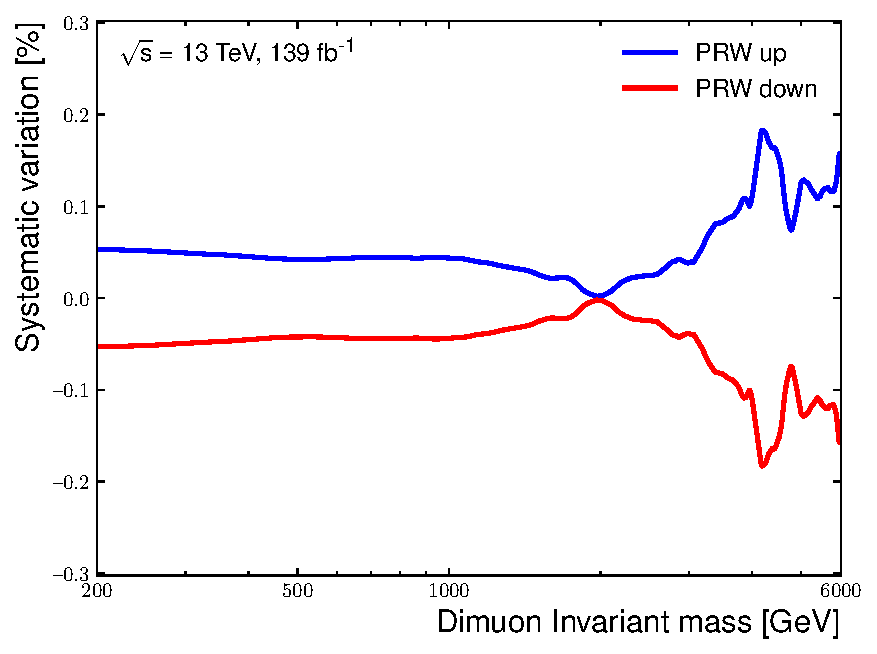
\includegraphics[width=\textwidth]{figures/analysis/datamc/Uncertainties/exp/mm/m_uu_pstOR_PRW_DATASF__1up.pdf}
        \label{fig:uncert:mmprw}
    \end{subfigure}
    \begin{subfigure}[h]{0.42\textwidth}
        \centering
        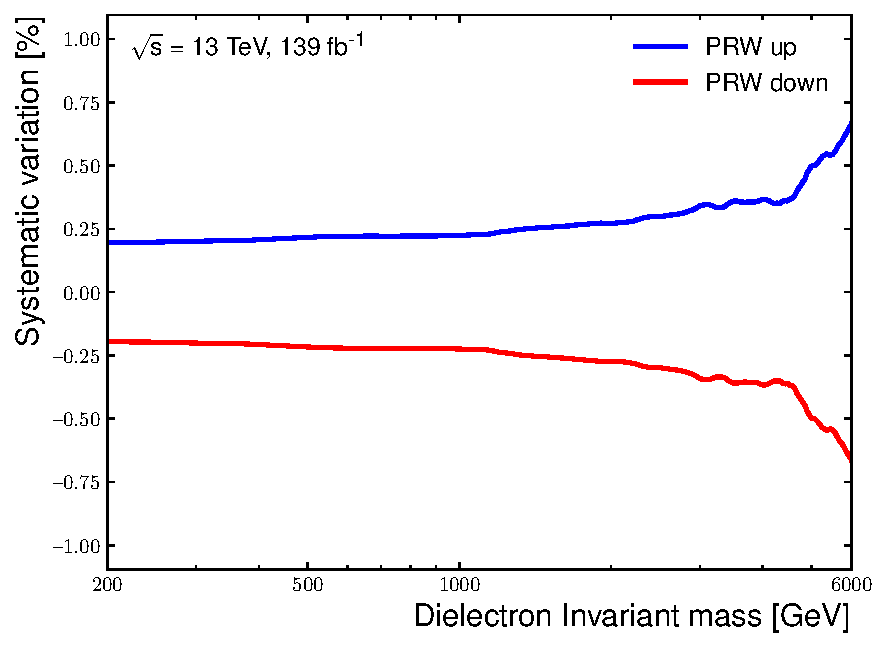
\includegraphics[width=\textwidth]{figures/analysis/datamc/Uncertainties/exp/ee/m_ee_pstOR_PRW_DATASF__1up.pdf}
        \label{fig:uncert:eeprw}
    \end{subfigure}
    \caption[Systematic uncertainty due to pileup reweighting]{Systematic uncertainties due to pileup in the muon (left) and electron (right).}
    \label{fig:uncert:prwuncert}
\end{figure}

\subsection{Lepton uncertainties}

\subsubsection{Efficiencies}
The electron and muon efficiency uncertainties are obtained by using the tag-and-probe method~\cite{Aaboud:2016vfy,Aad:2016jkr} by varying the selection of reconstruction, identification, isolation and trigger criteria individually~\cite{Aad:2019tso,Aad:2016jkr}. The tag-and-probe method uses $Z\rightarrow \ell\ell$ samples, where events are elected with pairs of leptons with opposite charge, that have an invariant mass in a window around the $Z$ peak. When one of the leptons passes the tight working point for the criteria above, it is taken as the \emph{tag} lepton, while the other is taken as the probe. The efficiency for a selection criteria can then be calculated by taking the number of probes which pass the tight selection over the total number of probes. Further detail on the efficiency uncertainty calculations are provided in \cite{Aad:2019tso,Aad:2016jkr} for electrons and muons, respectively. 

The systematic variations for reconstruction, isolation and identification are shown in \cref{fig:uncert:eeExp,fig:uncert:mmExp}. The isolation efficiency systematic variation for both the electron and muon channels are less than 1\%. The identification efficiency systematic variation for the electron channel increases from 2\% at low-mass to 4\% at high-mass. Whereas, for the muon channel the identification systematic variation is $< 1\%$ at low invariant masses with a sharp jump to 20\% at high-mass, resulting in a dramatic change in the shape of the invariant-mass distribution. The reconstruction efficiency variation for the electron channel follows a similar shape to the identification with a negligible impact <0.1\%. In the muon channel the reconstruction efficiency has a larger impact on the shape of the invariant-mass distribution with the uncertainty ranging from 2\% at low-mass to 30\% at high-mass. For both the electron and muon channels there is a negligible contribution from the trigger efficiency systematic variation, with a flat contribution < 0.001\% throughout the entire invariant-mass spectrum considered. Therefore, it is not included in the figure. 

\subsubsection{Resolution}
Smearing of the electron energies in MC accounts for the differences in energy resolution between data and MC. A full correlation model for energy resolution uncertainty consists of several nuisance parameters where all uncertainties have been decorrelated in bins of $\eta$~\cite{Aad:2019tso}.

The muon resolution corrections are calculated by fitting several correction coefficients that are used to match the invariant mass distributions between MC and data. Each fit parameter in the model is associated with a source of potential disagreement between data. The uncertainty on the resolution is derived by taking the variations of the fit procedure, the background parameterisation and muon spectrometer alignment~\cite{Aad:2016jkr}. 

The systematic variations for the resolution uncertainty in the electron and muon channel is shown in \cref{fig:uncert:eeExp,fig:uncert:mmExp}. The muon resolution is <1\% at low invariant masses up to \SI{2000}{\giga\electronvolt} with a sharp increase up to 28\% at \SI{6000}{\giga\electronvolt}. Whereas, the electron resolution uncertainty follows a similar shape, but with a much smaller impact, ranging from <0.1\% at low invariant mass to 0.75\% at \SI{6000}{\giga\electronvolt}. The uncertainty in both channel will result in a sharp change in the shape of the invariant-mass distribution. However, the effect is significantly larger in the muon channel. 

\cref{fig:uncert:mass_resolution_eemm} depicts the dielectron and dimuon mass resolution as a function of the generated mass of the dilepton pair. In contrast to the dielectron channel, it can be seen in the dimuon channel that the mass resolution significantly deteriorates at higher invariant-mass. The impact of the muon resolution uncertainty on the data-driven extrapolation method, discussed in \cref{chap:uncertBkgmodel}, was studied in detail. In particular, the impact of increasing the muon resolution uncertainty on the data-driven uncertainties was studied. It was concluded that there is negligible impact on the data-driven uncertainties when the muon resolution uncertainty is increased by 90\% of it's initial value. This indicates that the functional form used is robust enough to take into account significant variations in the measurement of the muon resolution. 
\begin{figure}[!htb]
    \centering
    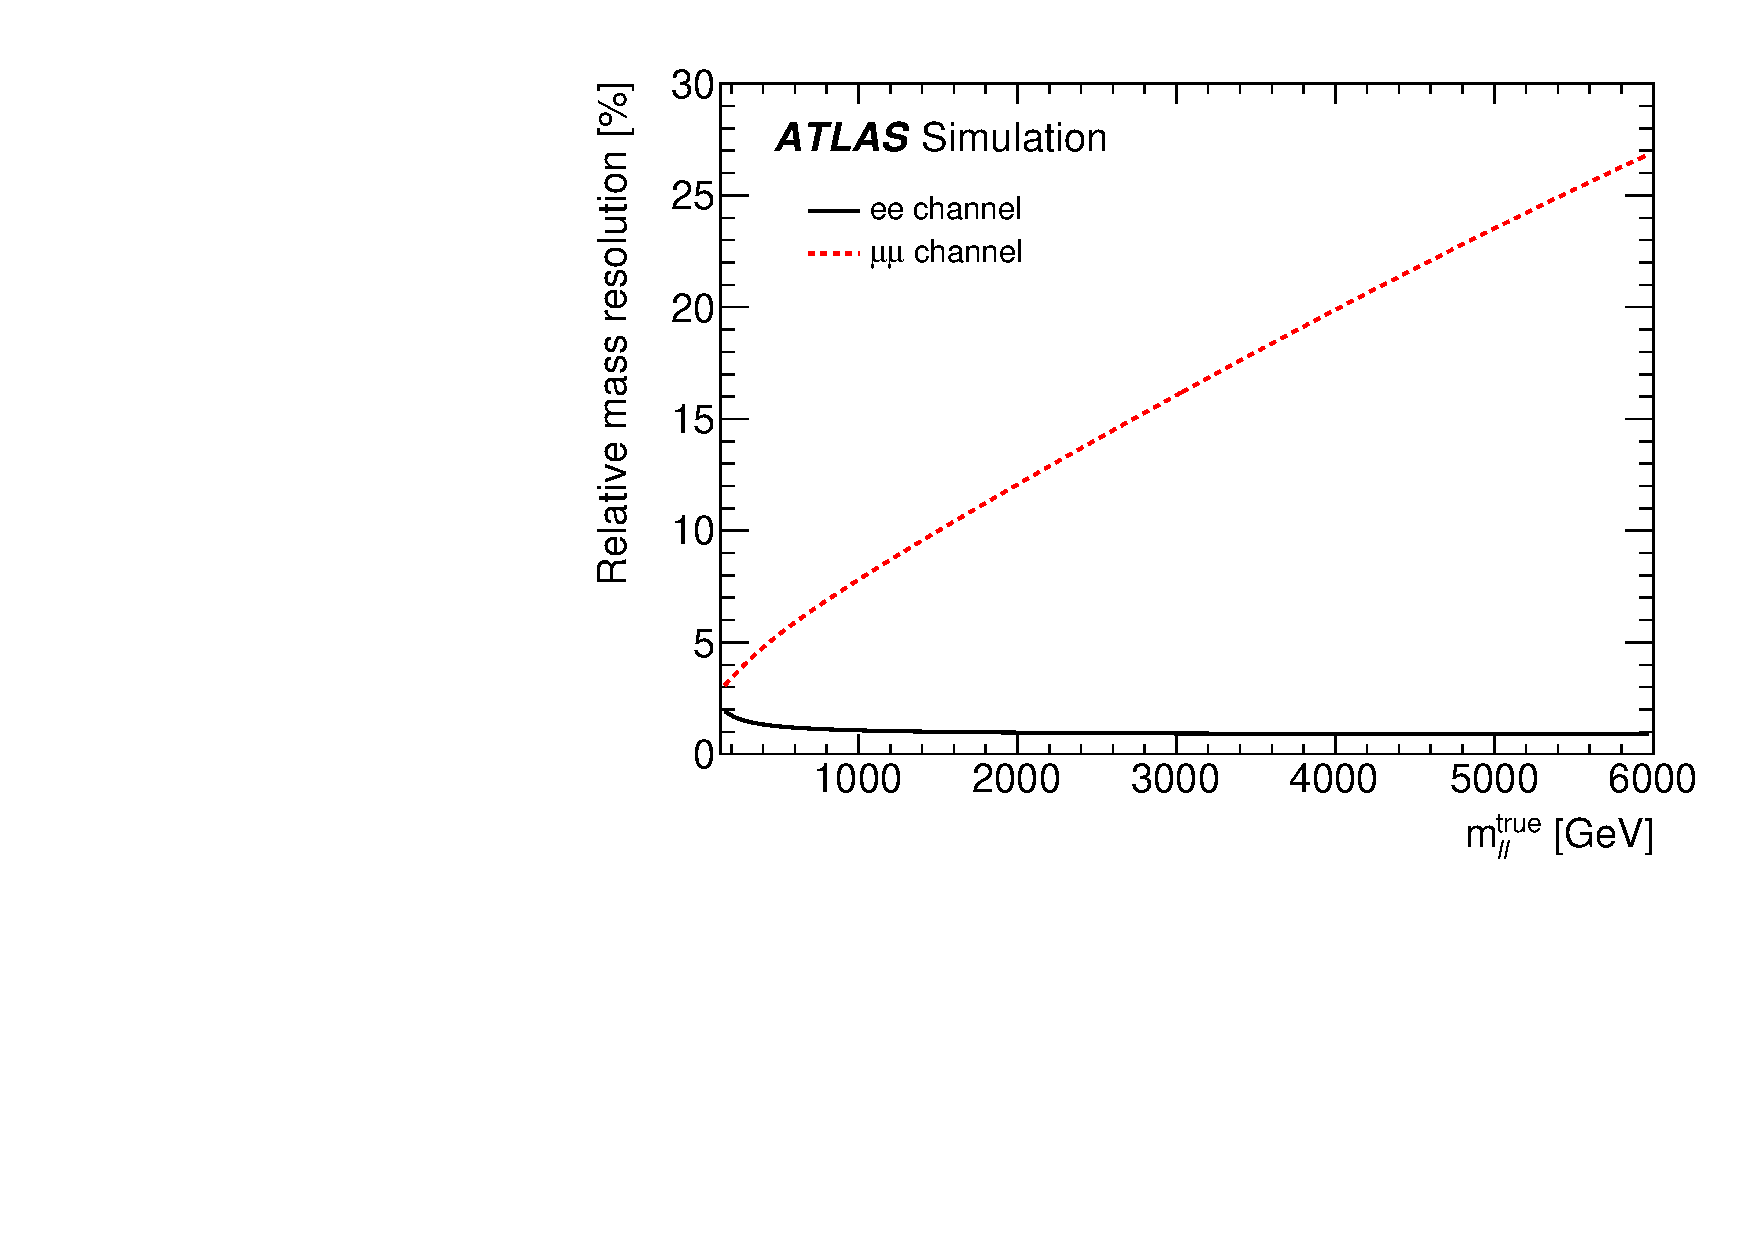
\includegraphics[width=\textwidth]{figures/analysis/datamc/Uncertainties/exp/figaux_15_massResolution.pdf}
    \caption[Dielectron and dimuon mass resolution as a function of the generated mass of the dilepton pair ($m_{\ell\ell}^{true}$)]{Dielectron and dimuon mass resolution as a function of the generated mass of the dilepton pair ($m_{\ell\ell}^{true}$)~\cite{Aad:2019fac}.}
    \label{fig:uncert:mass_resolution_eemm}
\end{figure}

\subsubsection{Energy scale}
Electron and muon energy scale corrections are applied only on data. The effects of varying the respective uncertainties associated with the energy scale corrections up and down is calculated to determine the systematic uncertainty. The resulting distributions are used to determine the systematic uncertainty and is calculated on MC due to the higher statistics available~\cite{Aad:2019tso}. 

\cref{fig:uncert:eeExp,fig:uncert:mmExp} show the size of the energy scale systematic variations. For the electron channel the uncertainty ranges from 0.35\% at low-mass to 0.65\% at high-mass. Whereas, for the muon channel the uncertainty is <0.1\% at low mass with a sharp increase to 15\% at high-mass. 

\begin{figure}[]
    \centering
    \begin{subfigure}[b]{0.42\textwidth}
        \centering
        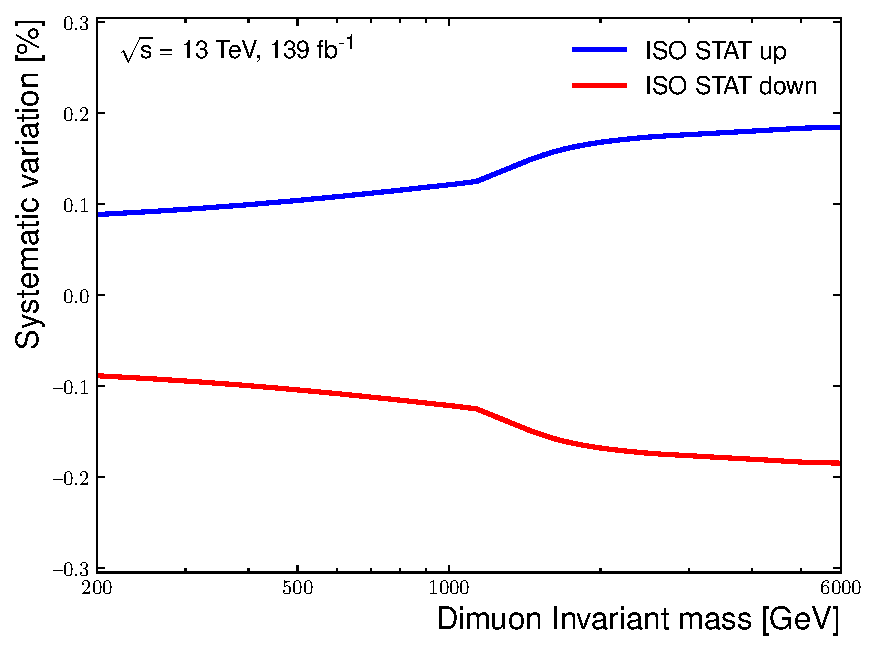
\includegraphics[width=\textwidth]{figures/analysis/datamc/Uncertainties/exp/mm/m_uu_pstOR_MUON_EFF_ISO_STAT__1up.pdf}
        \caption{}
        \label{fig:uncert:mmIso}
    \end{subfigure}
    \begin{subfigure}[b]{0.42\textwidth}
        \centering
        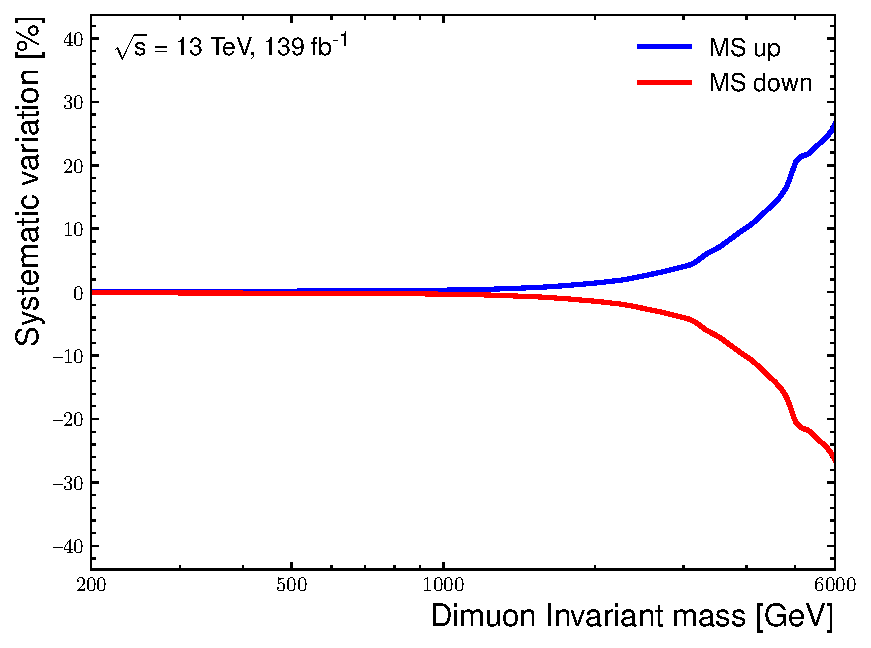
\includegraphics[width=\textwidth]{figures/analysis/datamc/Uncertainties/exp/mm/m_uu_pstOR_MUON_MS__1up.pdf}
        \caption{}
        \label{fig:uncert:mmMC}
    \end{subfigure}
    \begin{subfigure}[b]{0.42\textwidth}
        \centering
        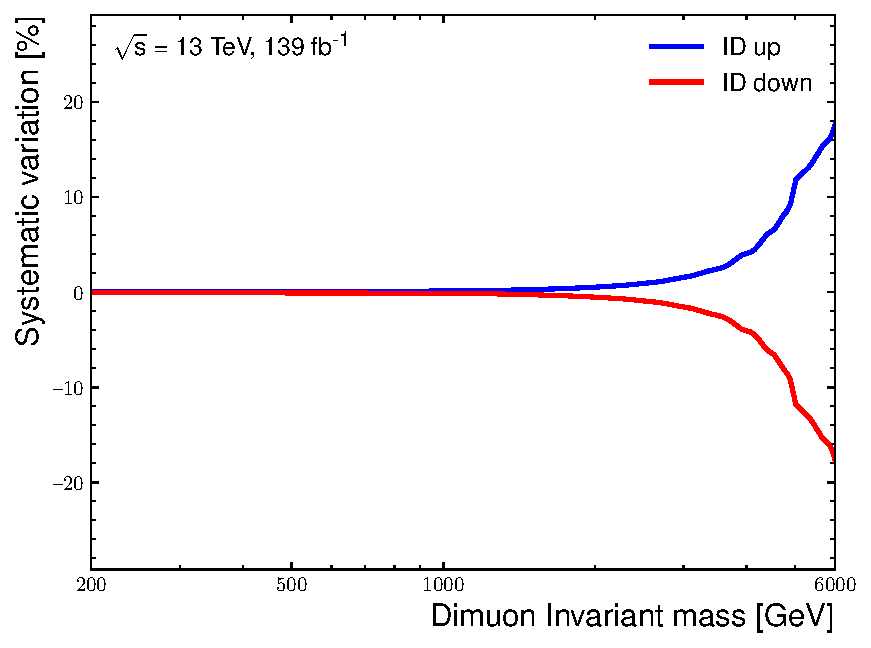
\includegraphics[width=\textwidth]{figures/analysis/datamc/Uncertainties/exp/mm/m_uu_pstOR_MUON_ID__1up.pdf}
        \caption{}
        \label{fig:uncert:mmID}
    \end{subfigure}
    % \begin{subfigure}[b]{0.42\textwidth}
    %     \centering
    %     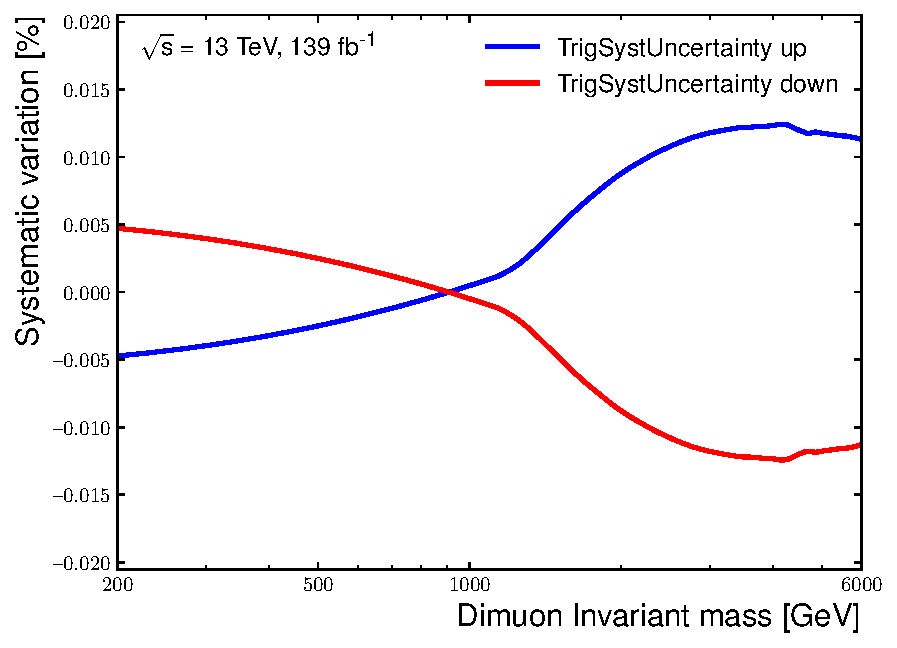
\includegraphics[width=\textwidth]{figures/analysis/datamc/Uncertainties/exp/mm/m_uu_pstOR_MUON_EFF_TrigSystUncertainty__1up.pdf}
    %     \label{fig:uncert:mmTrig}
    % \end{subfigure}
    \begin{subfigure}[b]{0.42\textwidth}
        \centering
        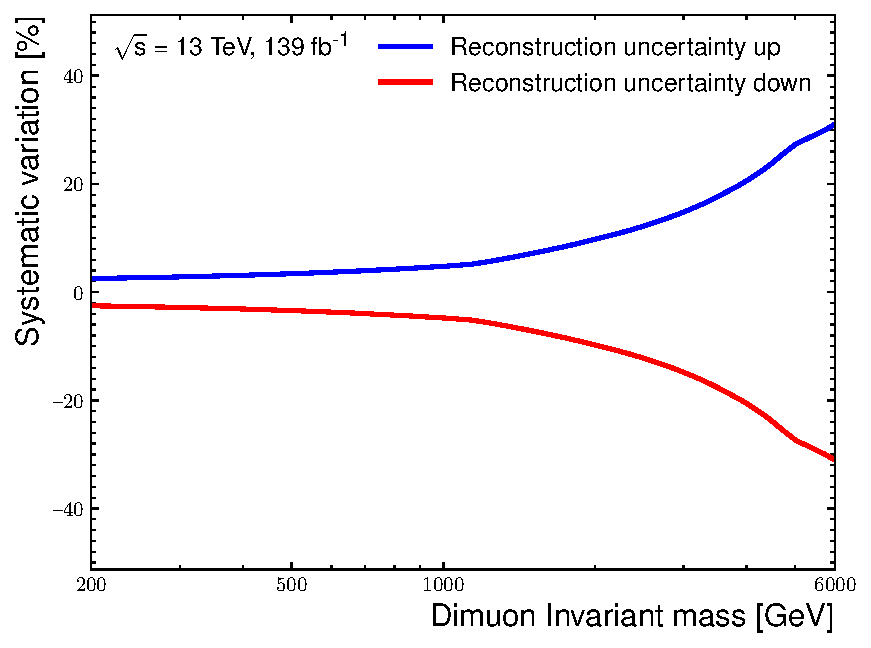
\includegraphics[width=\textwidth]{figures/analysis/datamc/Uncertainties/exp/mm/m_uu_pstOR_MUON_EFF_RECO_SYS__1up.pdf}
        \caption{}
        \label{fig:uncert:mmReco}
    \end{subfigure}
    \begin{subfigure}[b]{0.42\textwidth}
        \centering
        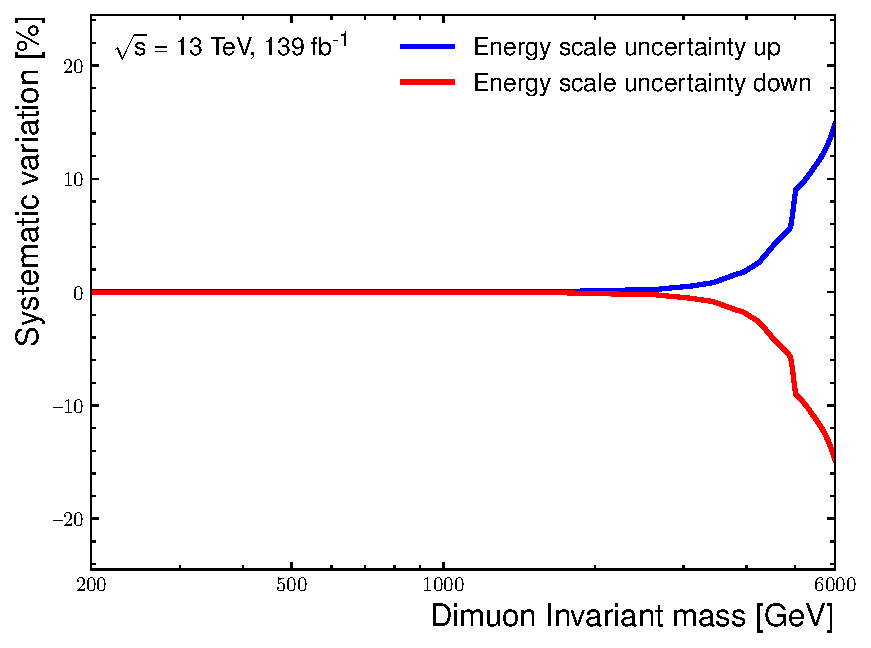
\includegraphics[width=\textwidth]{figures/analysis/datamc/Uncertainties/exp/mm/m_uu_pstOR_MUON_SCALE__1up.pdf}
        \caption{}
        \label{fig:uncert:mmScale}
    \end{subfigure}
    \caption[Muon systematic uncertainties due to experimental sources]{Muon systematic uncertainties due to experimental sources. The uncertainty related to isolation (a), momentum resolution in the muon spectrometer (b) and inner detector (c), muon reconstruction (d), and muon energy scale (e) are shown.}
    \label{fig:uncert:mmExp}
\end{figure}

\begin{figure}[]
    \centering
    \begin{subfigure}[b]{0.42\textwidth}
        \centering
        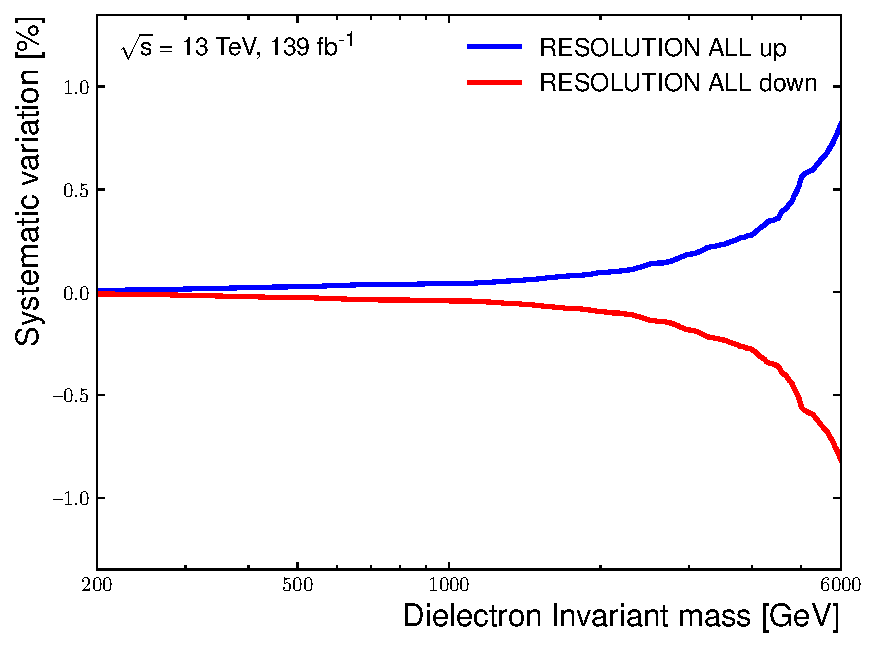
\includegraphics[width=\textwidth]{figures/analysis/datamc/Uncertainties/exp/ee/m_ee_pstOR_EG_RESOLUTION_ALL__1up.pdf}
        \caption{}
        \label{fig:uncert:eeRes}
    \end{subfigure}
    \begin{subfigure}[b]{0.42\textwidth}
        \centering
        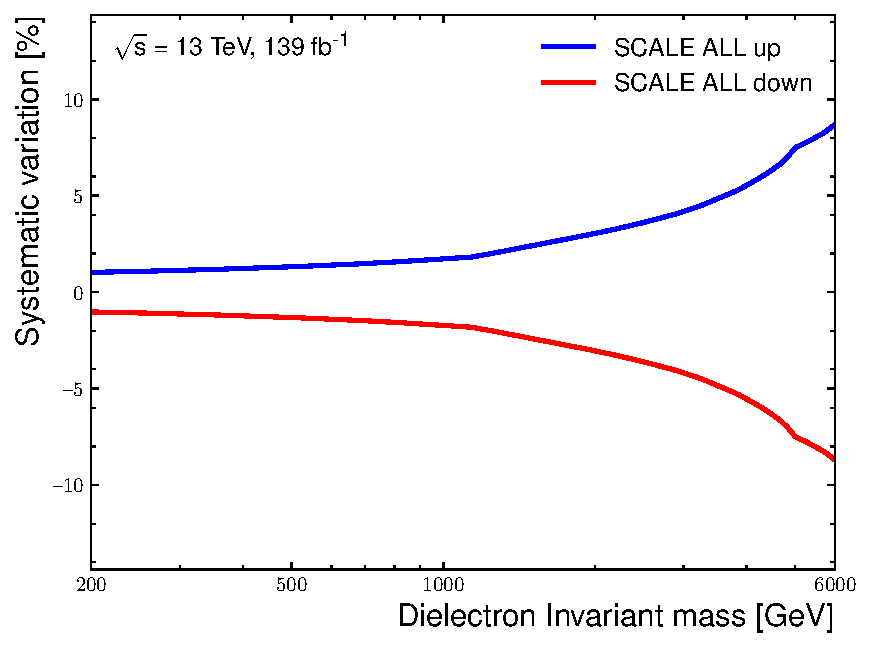
\includegraphics[width=\textwidth]{figures/analysis/datamc/Uncertainties/exp/ee/m_ee_pstOR_EG_SCALE_ALL__1up.pdf}
        \caption{}
        \label{fig:uncert:eeScale}
    \end{subfigure}
    \begin{subfigure}[b]{0.42\textwidth}
        \centering
        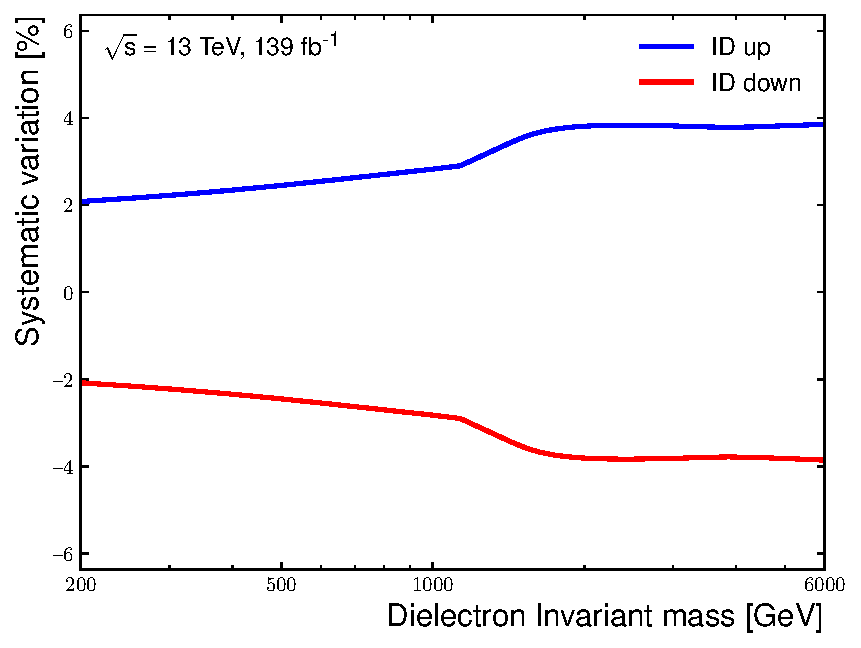
\includegraphics[width=\textwidth]{figures/analysis/datamc/Uncertainties/exp/ee/m_ee_pstOR_EL_EFF_ID_TOTAL_1NPCOR_PLUS_UNCOR__1up.pdf}
        \caption{}
        \label{fig:uncert:eeID}
    \end{subfigure}
    \begin{subfigure}[b]{0.42\textwidth}
        \centering
        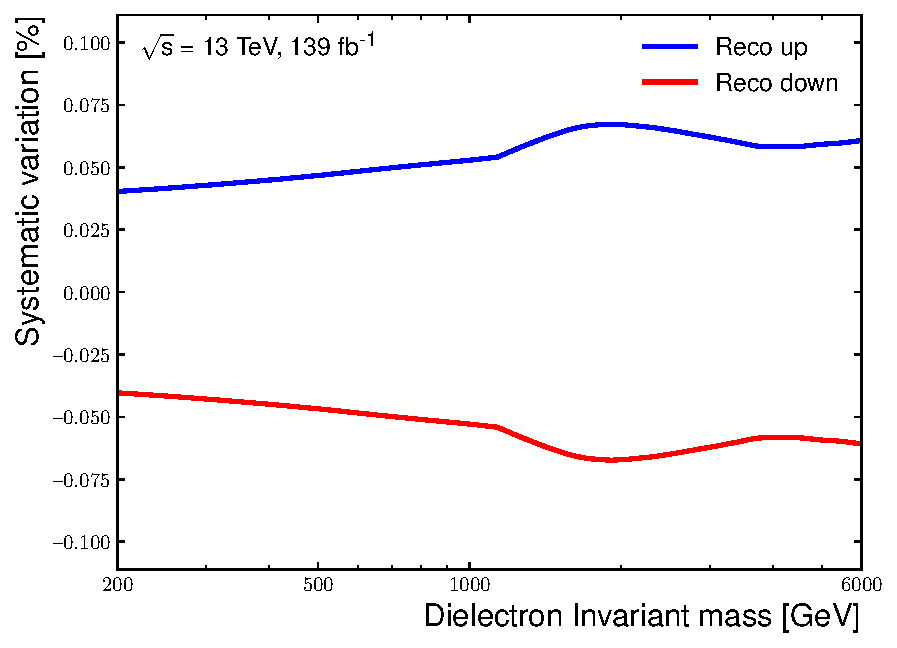
\includegraphics[width=\textwidth]{figures/analysis/datamc/Uncertainties/exp/ee/m_ee_pstOR_EL_EFF_Reco_TOTAL_1NPCOR_PLUS_UNCOR__1up.pdf}
        \caption{}
        \label{fig:uncert:eeReco}
    \end{subfigure}
    \begin{subfigure}[b]{0.42\textwidth}
        \centering
        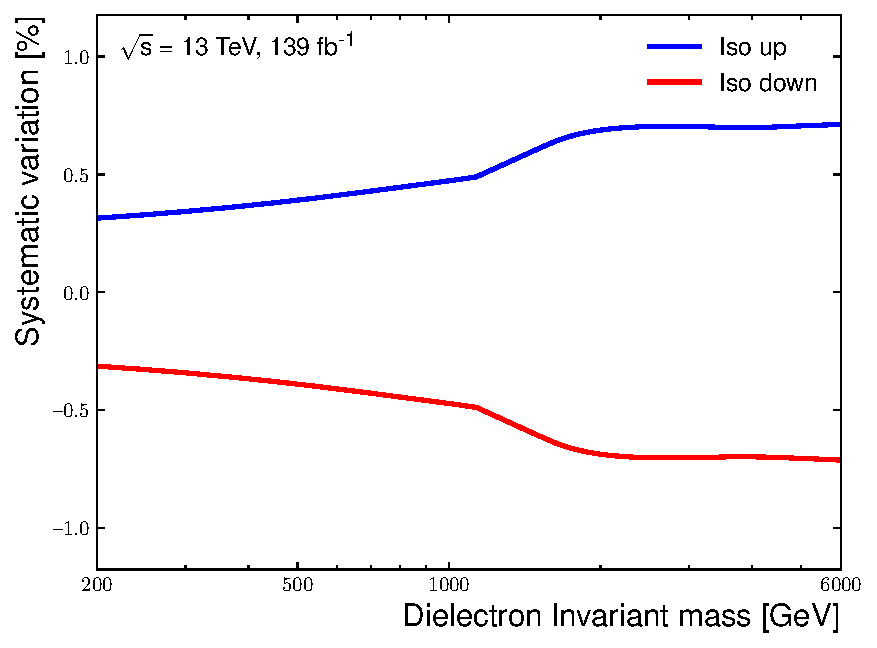
\includegraphics[width=\textwidth]{figures/analysis/datamc/Uncertainties/exp/ee/m_ee_pstOR_EL_EFF_Iso_TOTAL_1NPCOR_PLUS_UNCOR__1up.pdf}
        \caption{}
        \label{fig:uncert:eeIso}
    \end{subfigure}
    % \begin{subfigure}[b]{0.42\textwidth}
    %     \centering
    %     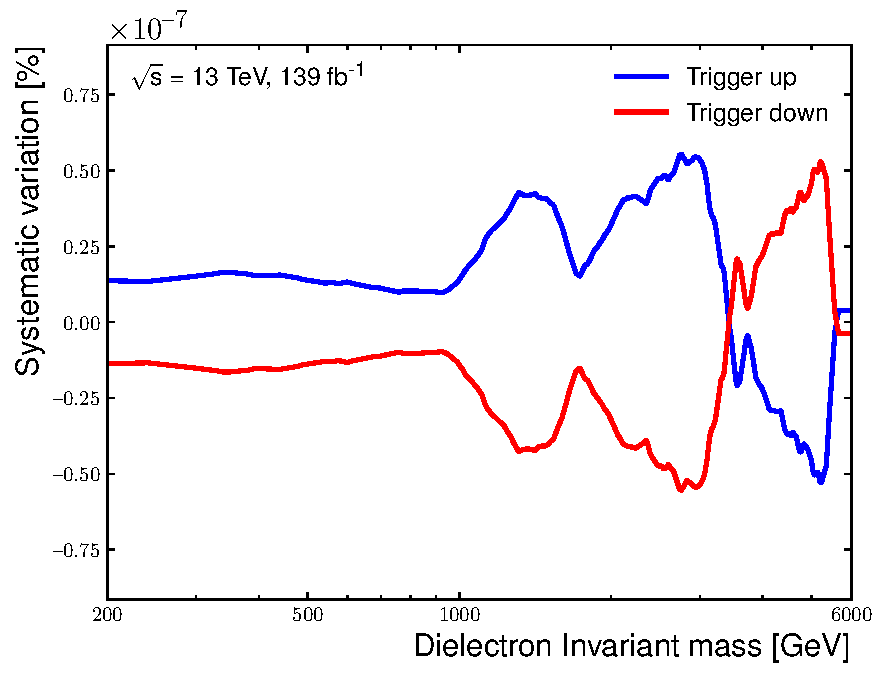
\includegraphics[width=\textwidth]{figures/analysis/datamc/Uncertainties/exp/ee/m_ee_pstOR_EL_EFF_Trigger_TOTAL_1NPCOR_PLUS_UNCOR__1up.pdf}
    %     \label{fig:uncert:eeTrig}
    % \end{subfigure}
    \caption[Electron systematic uncertainties due to experimental sources]{Electron systematic uncertainties due to experimental sources. The uncertainty related to electron energy resolution (a), energy scale (b), identification (c), reconstruction (d) and isolation (e) are shown.}
    \label{fig:uncert:eeExp}
\end{figure}

\section{Theoretical uncertainties}\label{sec:sysmc:theory}
The theoretical uncertainties on the simulated samples are only used to determine the uncertainty of the background modelling. High-energy searches like the one described in this thesis probe previously uncharted kinematic regions as their mass predictions extend to \SI{}{\tera\electronvolt} energy scales. Therefore, a detailed understanding of systematic uncertainties related to the knowledge of the partonic structure of the proton is required. The kinematic range probed extends beyond the range where the PDF is calculated from in data. The uncertainties related to the PDF are separated into those which arise from the variations of the eigenvectors fo the PDF, the choice of the PDF with respect to other available PDFs, referred to as PDF choice uncertainty, and the scale uncertainties associated with the EW and and strong coupling constants. Additionally, the uncertainty on the top-quark and diboson background is also summarised in below. 

% \subsection{PDF uncertainties}
\subsubsection{PDF eigenvector uncertainties}
The PDF uncertainties are studied for the leading DY background. Each available PDF has a set of independent parameters known as eigenvectors associated with it. These eigenvectors can be varied in orthogonal directions to quantify systematic uncertainties associated with a PDF set. For each eigenvector variation at the 90\% Confidence Level in the CT10NNLO~\cite{ct10} parameterisation, the DY cross-section is calculated at NNLO as a function of $m_{\ell\ell}$. The eigenvector variation uncertainty is taken as the relative deviation of the cross-sections of the PDF resulting from the eigenvector variations and the nominal PDF. For each $m_{\ell\ell}$ bin in a histogram, the asymmetric uncertainty on the cross-section is obtained using
\begin{equation}
    \begin{aligned}
    \Delta \sigma^+ = \sqrt{\sum^n_{i=1}\mathrm{Max}\left(\sigma_i^+ - \sigma_0, \sigma^-_i - \sigma_0,0     \right)}, \\
    \Delta \sigma^- = \sqrt{\sum^n_{i=1}\mathrm{Max}\left(\sigma_0 - \sigma_i^+, \sigma_0 -\sigma^-_i,0  \right)}, \\
    \end{aligned}
\end{equation}
where n is the number of PDF eigenvectors, $\sigma_i^{+/-}$ is the cross-section for the higher and lower values for the corresponding PDF eigenvector variation, and $\sigma_0$ is the cross-section for the central value for the PDF. A total of seven eigenvector variations are considered in this analysis. The total asymmetric uncertainty at each invariant mass bin is calculated using the above equation. The effects of the PDF eigenvector variations is shown in \cref{fig:ucnert:eepdfvar,fig:ucnert:mmpdfvar}. The eigenvector variations result in large changes in the shape of the invariant-mass distributions. The uncertainties show a large increase at high invariant-masses indicating the poor theoretical understanding of the PDF in the high-energy regime.

\begin{figure}[h!]
    \centering
    \begin{subfigure}[b]{0.42\textwidth}
        \centering
        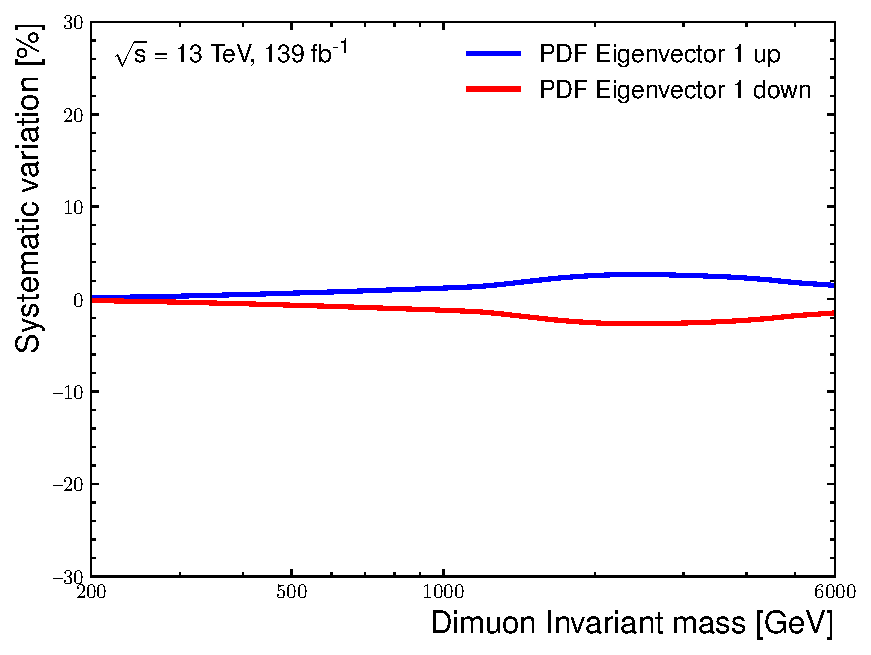
\includegraphics[width=\textwidth]{figures/analysis/datamc/Uncertainties/theory/mm/backgroundTemplate_KF_PDF_EV1.pdf}
        \label{fig:uncert:mmpdfvar1}
    \end{subfigure}
    \begin{subfigure}[b]{0.42\textwidth}
        \centering
        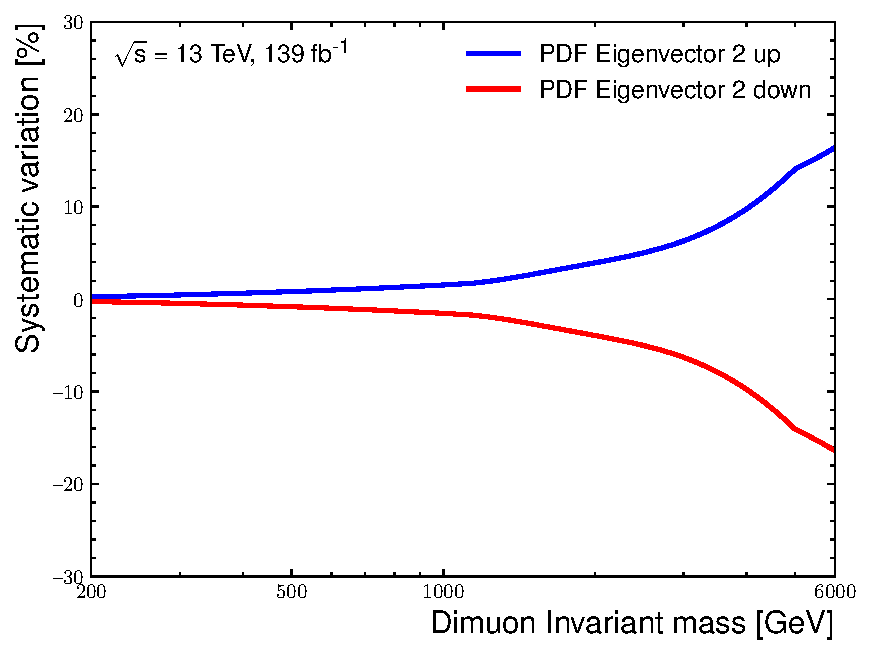
\includegraphics[width=\textwidth]{figures/analysis/datamc/Uncertainties/theory/mm/backgroundTemplate_KF_PDF_EV2.pdf}
        \label{fig:uncert:mmpdfvar2}
    \end{subfigure}
    \begin{subfigure}[b]{0.42\textwidth}
        \centering
        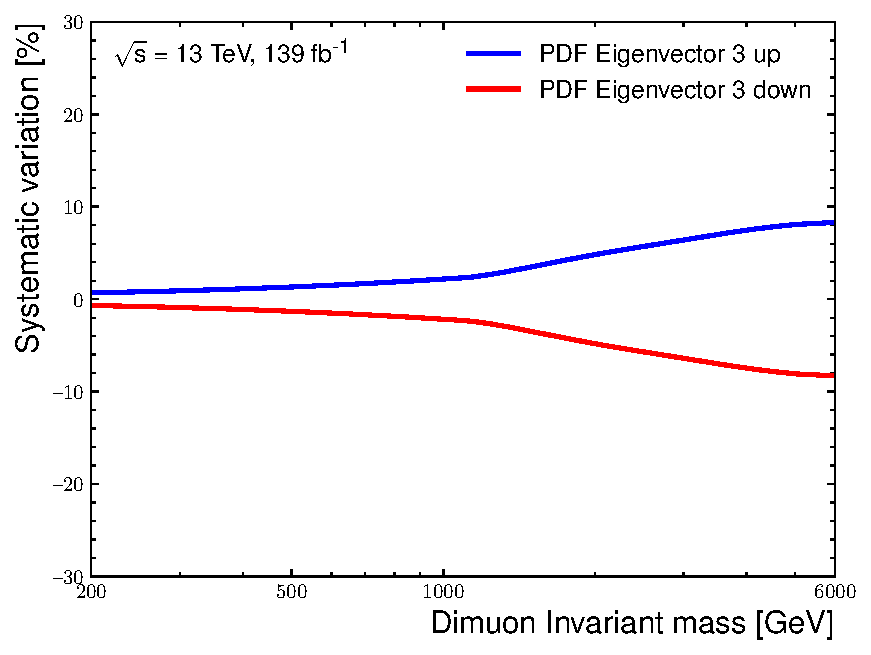
\includegraphics[width=\textwidth]{figures/analysis/datamc/Uncertainties/theory/mm/backgroundTemplate_KF_PDF_EV3.pdf}
        \label{fig:uncert:mmpdfvar3}
    \end{subfigure}
    \begin{subfigure}[b]{0.42\textwidth}
        \centering
        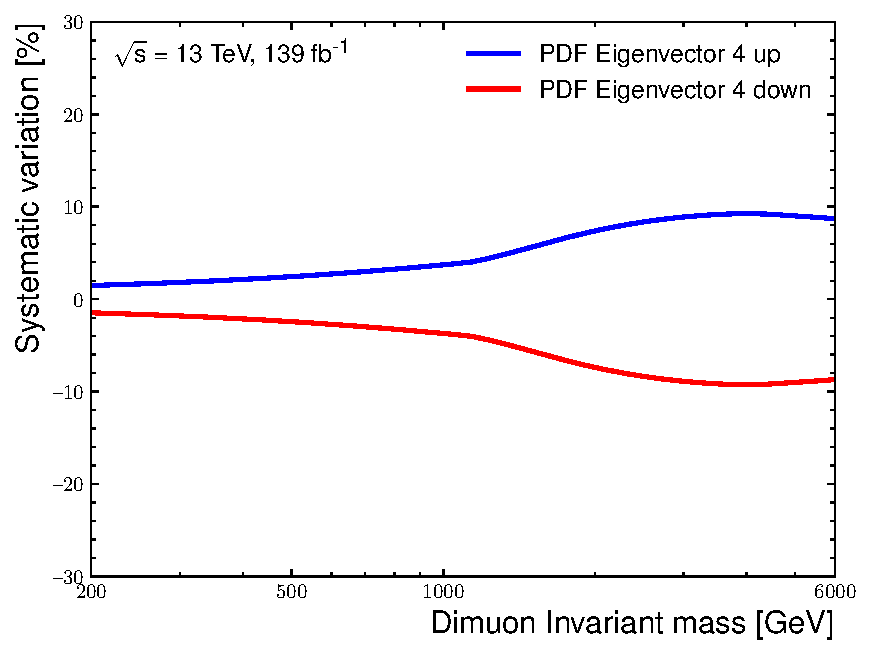
\includegraphics[width=\textwidth]{figures/analysis/datamc/Uncertainties/theory/mm/backgroundTemplate_KF_PDF_EV4.pdf}
        \label{fig:uncert:mmpdfvar4}
    \end{subfigure}
    \begin{subfigure}[b]{0.42\textwidth}
        \centering
        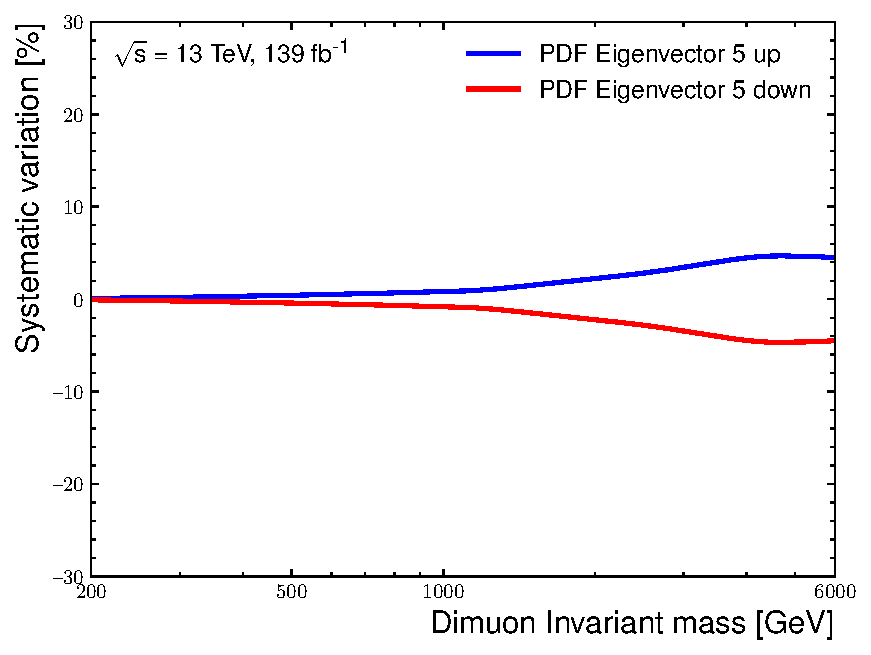
\includegraphics[width=\textwidth]{figures/analysis/datamc/Uncertainties/theory/mm/backgroundTemplate_KF_PDF_EV5.pdf}
        \label{fig:uncert:mmpdfvar5}
    \end{subfigure}
    \begin{subfigure}[b]{0.42\textwidth}
        \centering
        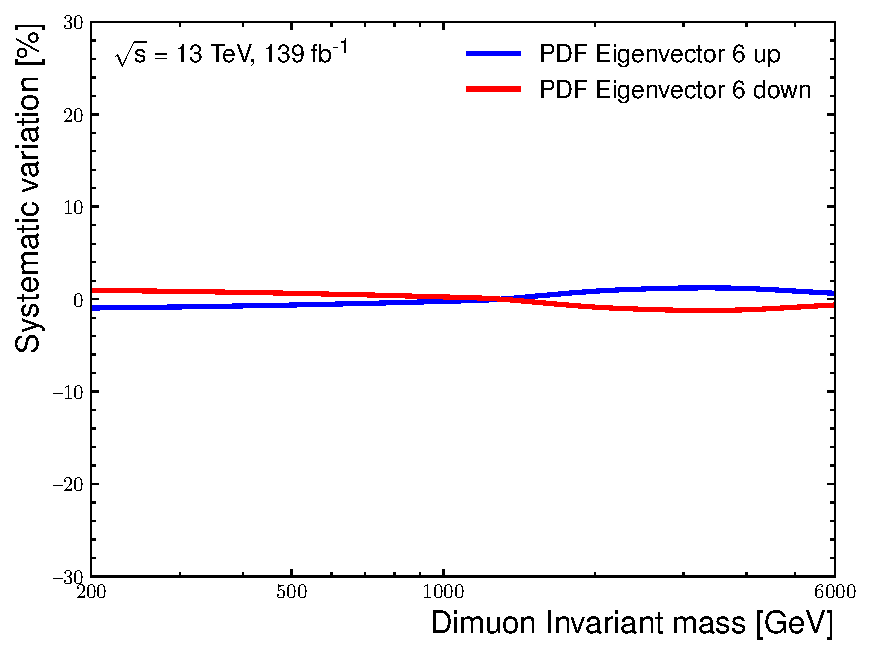
\includegraphics[width=\textwidth]{figures/analysis/datamc/Uncertainties/theory/mm/backgroundTemplate_KF_PDF_EV6.pdf}
        \label{fig:uncert:mmpdfvar6}
    \end{subfigure}
    \begin{subfigure}[b]{0.42\textwidth}
        \centering
        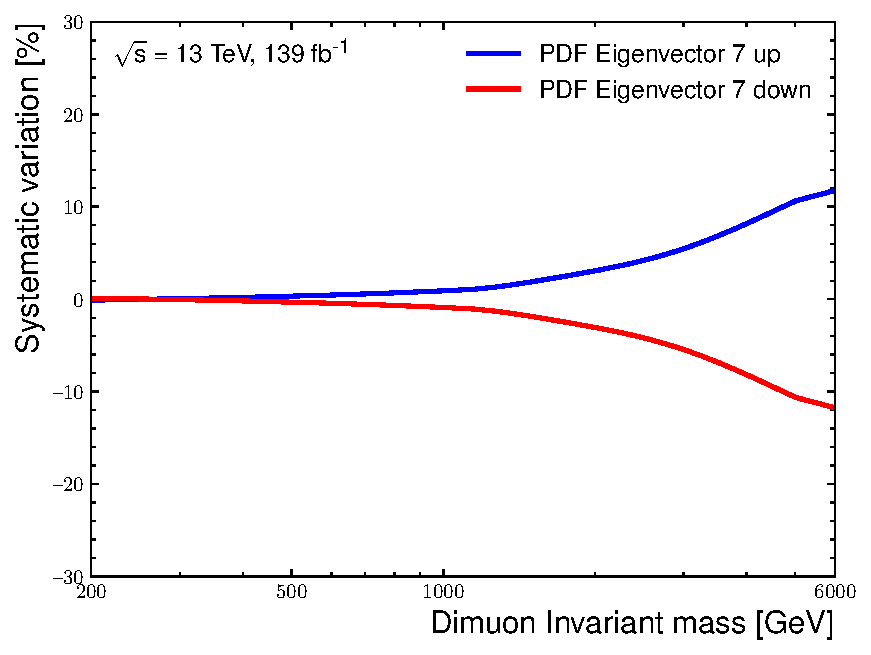
\includegraphics[width=\textwidth]{figures/analysis/datamc/Uncertainties/theory/mm/backgroundTemplate_KF_PDF_EV7.pdf}
        \label{fig:uncert:mmpdfvar7}
    \end{subfigure}
    \caption{Systematic uncertainties due to theoretical sources in the muon channel. The uncertainties corresponding to the seven eigenvector variations of the CT10NNLO PDF are shown in the figure.}
    \label{fig:ucnert:mmpdfvar}
\end{figure}

\begin{figure}[h!]
    \centering
    \begin{subfigure}[b]{0.42\textwidth}
        \centering
        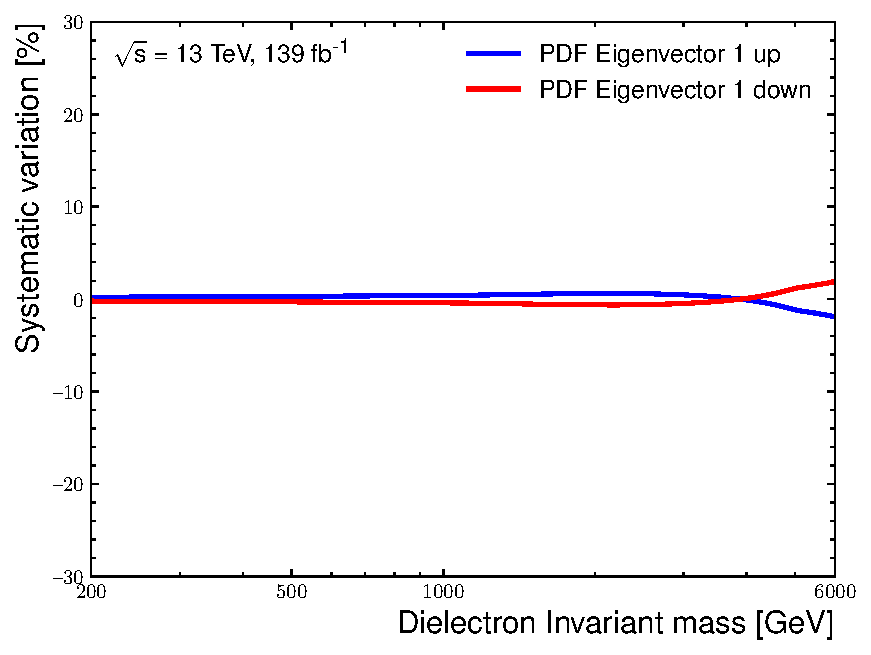
\includegraphics[width=\textwidth]{figures/analysis/datamc/Uncertainties/theory/ee/backgroundTemplate_KF_PDF_EV1.pdf}
        \label{fig:uncert:eepdfvar1}
    \end{subfigure}
    \begin{subfigure}[b]{0.42\textwidth}
        \centering
        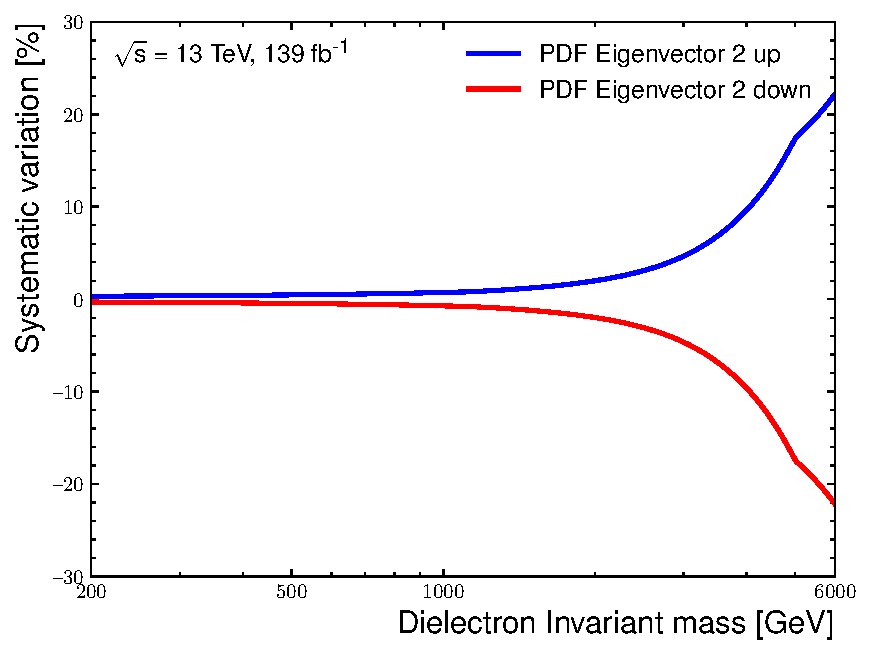
\includegraphics[width=\textwidth]{figures/analysis/datamc/Uncertainties/theory/ee/backgroundTemplate_KF_PDF_EV2.pdf}
        \label{fig:uncert:eepdfvar2}
    \end{subfigure}
    \begin{subfigure}[b]{0.42\textwidth}
        \centering
        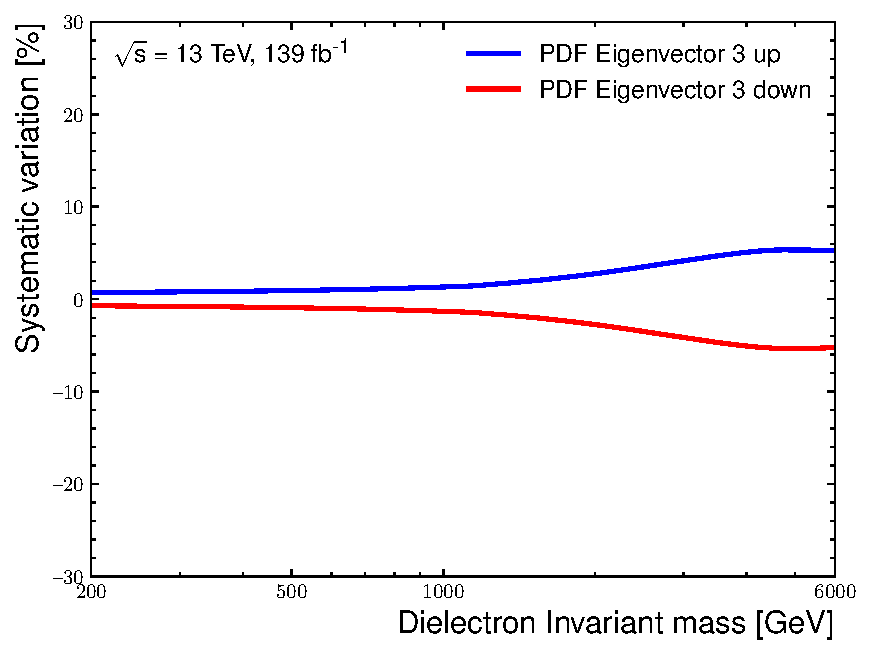
\includegraphics[width=\textwidth]{figures/analysis/datamc/Uncertainties/theory/ee/backgroundTemplate_KF_PDF_EV3.pdf}
        \label{fig:uncert:eepdfvar3}
    \end{subfigure}
    \begin{subfigure}[b]{0.42\textwidth}
        \centering
        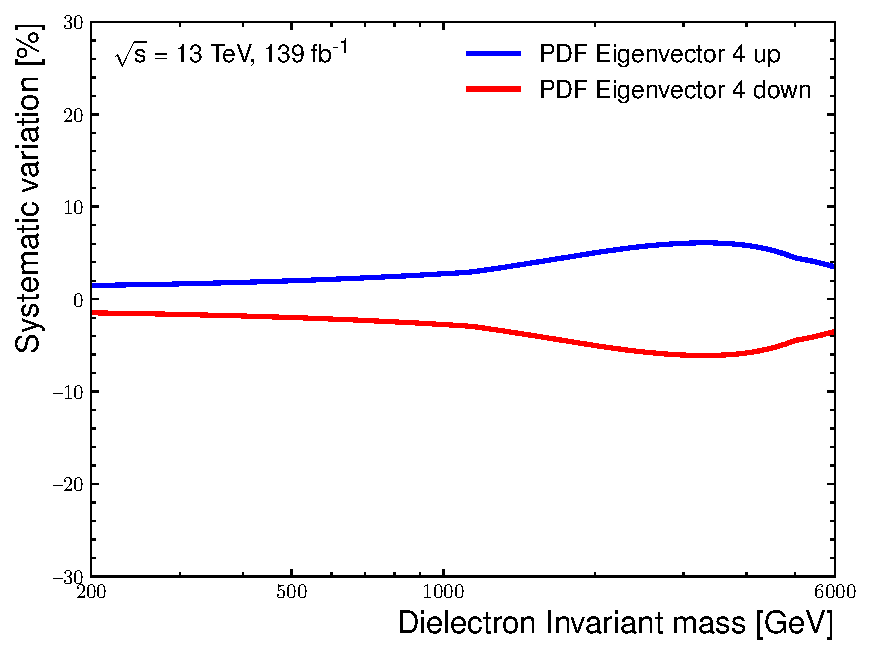
\includegraphics[width=\textwidth]{figures/analysis/datamc/Uncertainties/theory/ee/backgroundTemplate_KF_PDF_EV4.pdf}
        \label{fig:uncert:eepdfvar4}
    \end{subfigure}
    \begin{subfigure}[b]{0.42\textwidth}
        \centering
        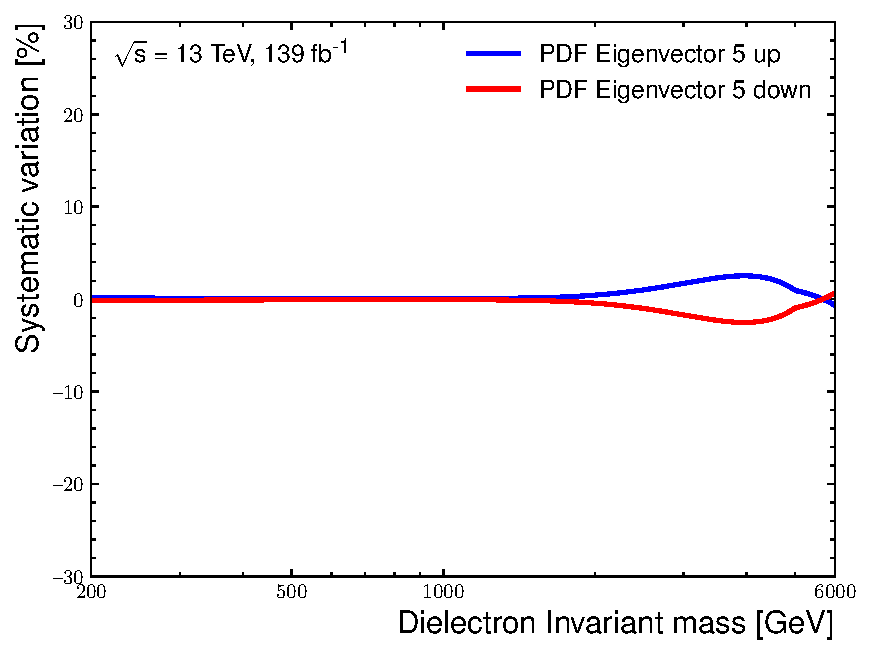
\includegraphics[width=\textwidth]{figures/analysis/datamc/Uncertainties/theory/ee/backgroundTemplate_KF_PDF_EV5.pdf}
        \label{fig:uncert:eepdfvar5}
    \end{subfigure}
    \begin{subfigure}[b]{0.42\textwidth}
        \centering
        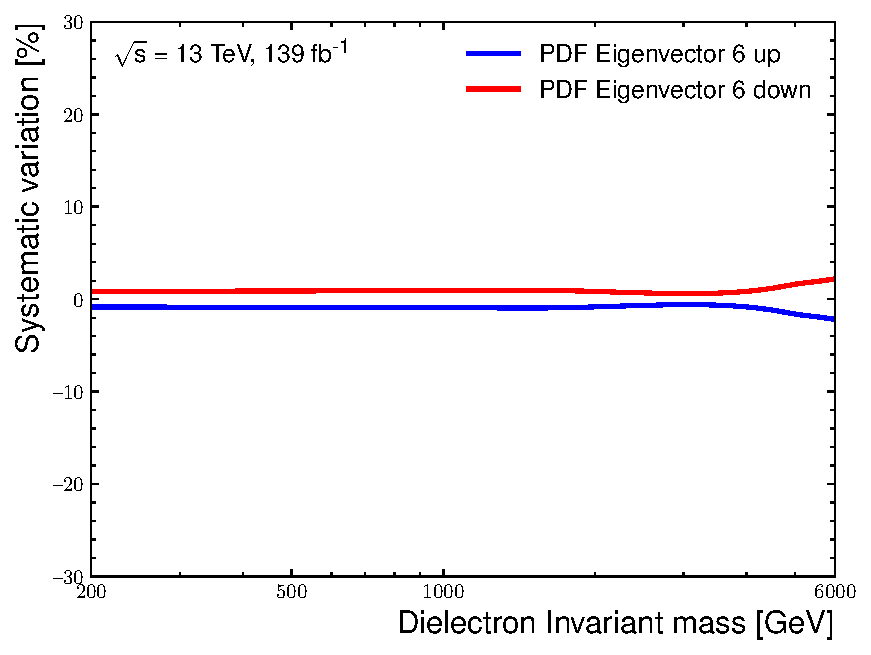
\includegraphics[width=\textwidth]{figures/analysis/datamc/Uncertainties/theory/ee/backgroundTemplate_KF_PDF_EV6.pdf}
        \label{fig:uncert:eepdfvar6}
    \end{subfigure}
    \begin{subfigure}[b]{0.42\textwidth}
        \centering
        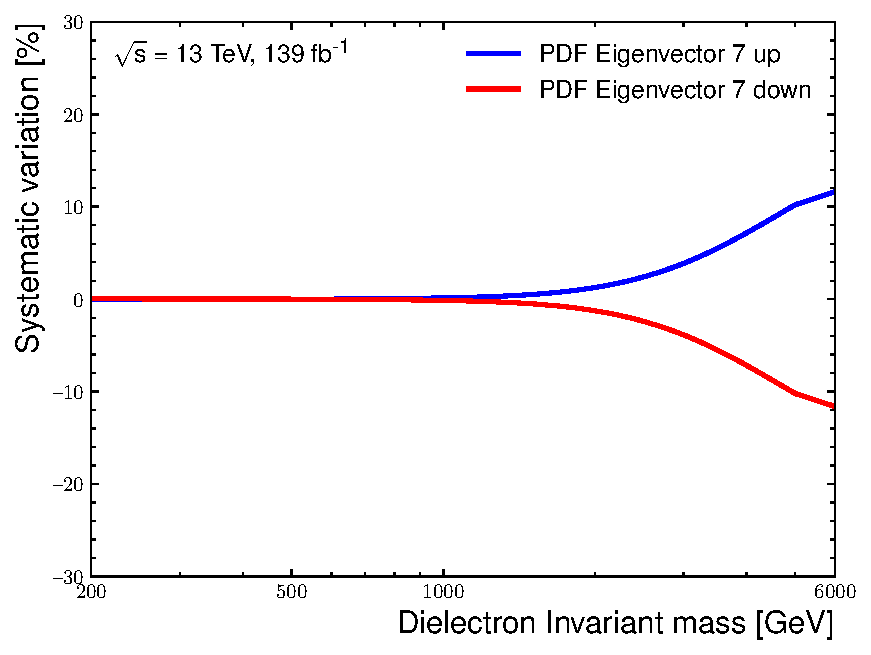
\includegraphics[width=\textwidth]{figures/analysis/datamc/Uncertainties/theory/ee/backgroundTemplate_KF_PDF_EV7.pdf}
        \label{fig:uncert:eepdfvar7}
    \end{subfigure}
    \caption{Systematic uncertainties due to theoretical sources in the electron channel. The uncertainties corresponding to the seven eigenvector variations of the CT10NNLO PDF are shown in the figure.}
    \label{fig:ucnert:eepdfvar}
\end{figure}

\subsubsection{PDF choice uncertainty}
The uncertainty related to the choice of PDF is determined by comparing the central value of CT10NNLO PDF to similar PDFs. Two alternatives for the nominal PDF are considered, the NNPDF3.0 and HERAPDF20 PDFs. At low masses $< \SI{3}{\tera\electronvolt}$ the PDF sets are in good agreement. At invariant masses $< \SI{3}{\tera\electronvolt}$ the PDF sets are in good agreement. However, at higher masses, the PDFs begin to diverge, with some PDF enveloped becoming very large. When the PDF difference between the nominal PDF and an alternative is larger than the uncertainty related to the PDF eigenvector variations, the maximum deviation of the envelope of the comparisons is taken as the PDF choice uncertainty. \cref{fig:uncert:pdfchoice} depicts the PDF choice uncertainty comparing the nominal PDF to NNPDF3.0 and HERAPDF20 in the electron and muon channels. The figure shows the agreement between the PDFs at low-masses, where the uncertainty is small, and a large increase at high invariant-mass indicating the point at which the PDFs start to diverge from their predictions. Similar to the PDF eigenvector uncertainties there is a significant change in shape of the uncertainties shown in the figure.

\begin{figure}[h!]
    \centering
    \begin{subfigure}[b]{0.42\textwidth}
        \centering
        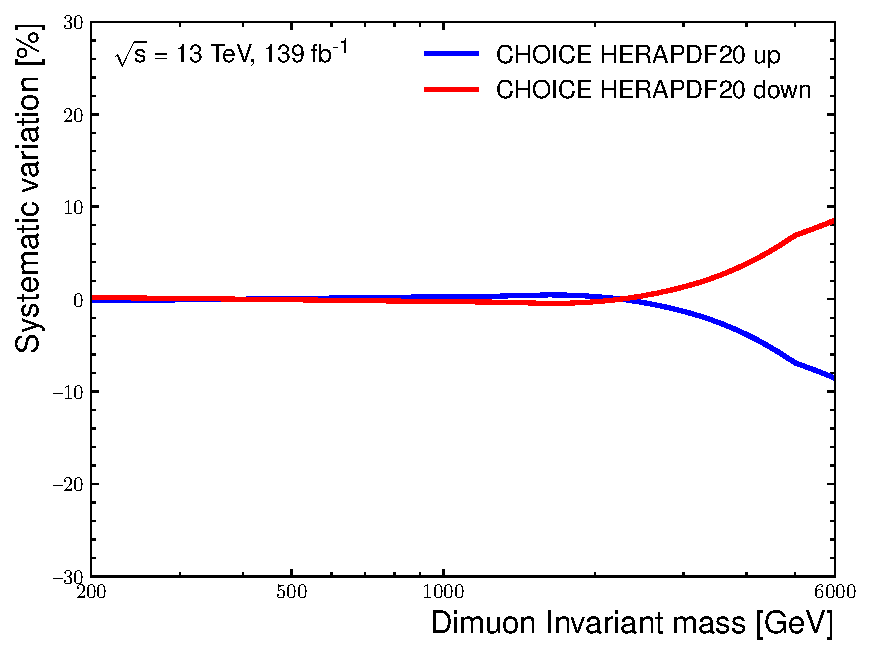
\includegraphics[width=\textwidth]{figures/analysis/datamc/Uncertainties/theory/mm/backgroundTemplate_KF_CHOICE_HERAPDF20.pdf}
        \caption{}
        \label{fig:uncert:mmchoiceHERA}
    \end{subfigure}
    \begin{subfigure}[b]{0.42\textwidth}
        \centering
        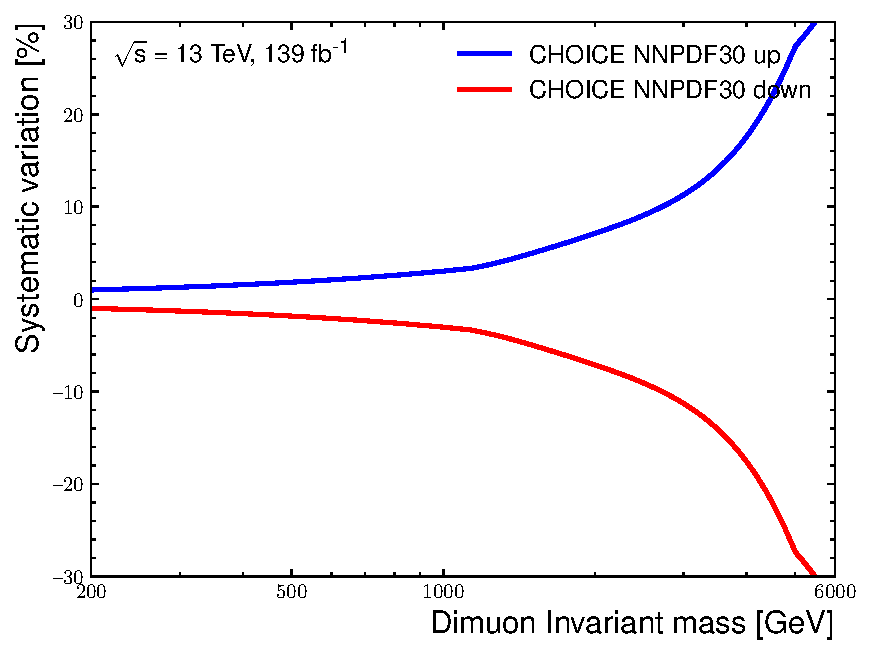
\includegraphics[width=\textwidth]{figures/analysis/datamc/Uncertainties/theory/mm/backgroundTemplate_KF_CHOICE_NNPDF30.pdf}
        \caption{}
        \label{fig:uncert:mmchoiceNNPDF}
    \end{subfigure}
    \begin{subfigure}[b]{0.42\textwidth}
        \centering
        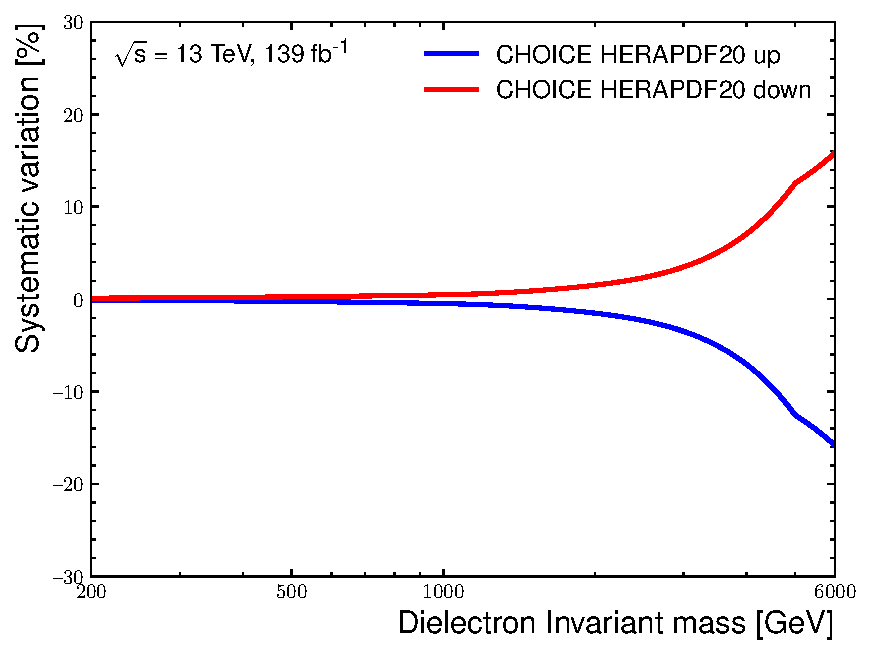
\includegraphics[width=\textwidth]{figures/analysis/datamc/Uncertainties/theory/ee/backgroundTemplate_KF_CHOICE_HERAPDF20.pdf}
        \caption{}
        \label{fig:uncert:eechoiceHERA}
    \end{subfigure}
    \begin{subfigure}[b]{0.42\textwidth}
        \centering
        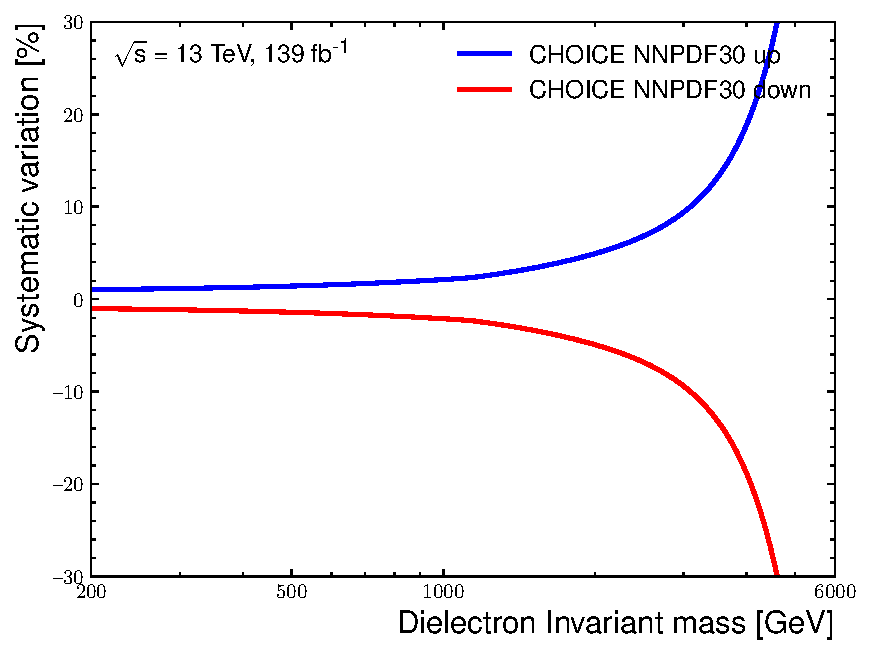
\includegraphics[width=\textwidth]{figures/analysis/datamc/Uncertainties/theory/ee/backgroundTemplate_KF_CHOICE_NNPDF30.pdf}
        \caption{}
        \label{fig:uncert:eechoiceNNPDF}
    \end{subfigure}
    \caption{Systematic uncertainties due to the choice of the nominal with respect to HERAPDF20 (a)/(b) and NNPDF30 (c)/(d) in the muon and electron channels, respectively.}
    \label{fig:uncert:pdfchoice}
\end{figure}

\subsubsection{PDF scale uncertainty}
The uncertainty on the PDF scales are calculated by varying the factorisation and renormalisation scales of the nominal PDF simultaneously by a factor of two. The resulting maximum variations are taken as the PDF scale uncertainties. \cref{fig:uncert:scales} shows the effects of the scale uncertainty on the invariant mass distribution for the electron and muon channels. 

\begin{figure}[h!]
    \centering
    \begin{subfigure}[h]{0.42\textwidth}
        \centering
        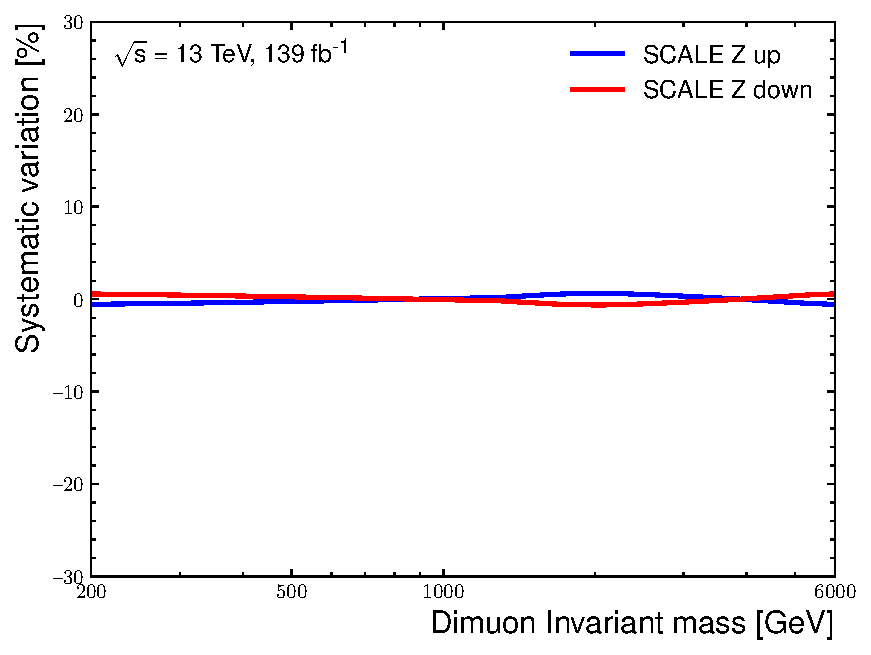
\includegraphics[width=\textwidth]{figures/analysis/datamc/Uncertainties/theory/mm/backgroundTemplate_KF_SCALE_Z__1up.pdf}
        \caption{}
        \label{fig:uncert:mmscaleZ}
    \end{subfigure}
    \begin{subfigure}[h]{0.42\textwidth}
        \centering
        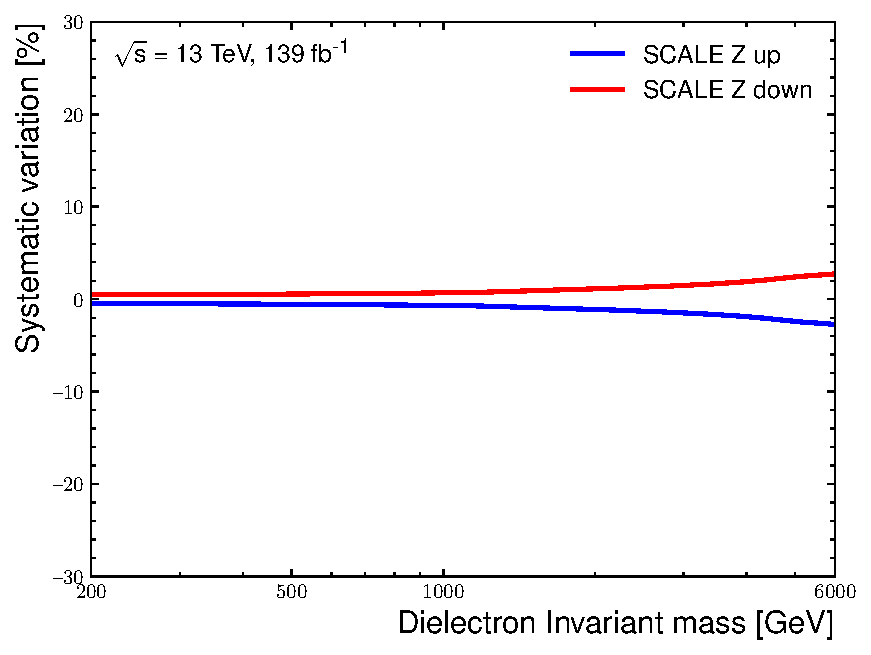
\includegraphics[width=\textwidth]{figures/analysis/datamc/Uncertainties/theory/ee/backgroundTemplate_KF_SCALE_Z__1up.pdf}
        \caption{}
        \label{fig:uncert:eescaleZ}
    \end{subfigure}
    \caption{Systematic uncertainties due to factorisation and renormalisation scales of the CT10NNLO PDF in the muon (a) and electron (b) channels.}
    \label{fig:uncert:scales}
\end{figure}

Uncertainties on the PDF also arise from the uncertainty of the strong coupling constant, $\alpha_s$. The uncertainty associated with  $\alpha_s$ is accounted for by studying the effect of changing $\alpha_s$ by $\pm 0.003$. The nominal value of 0.118 is taken for $\alpha_s$ in the cross-section calculation~\cite{Butterworth_2016}.

The combination of EW and QCD corrections is not fully known. Therefore, the EW correction systematic uncertainty was calculated by comparing the additive ($1 + \delta_{EW} + \delta_{QCD}$) versus factored ($(1 + \delta_{EW})(1 + \delta_{QCD})$) computation of the EW \emph{k}-factor. The difference between the two methods is taken as the uncertainty. The additive computation is used to obtain the nominal invariant mass distribution used in the search. 

\cref{fig:uncert:theoryConstants} show the uncertainties due to the EW and strong coupling constant on the invariant mass distributions for the electron and muon channels. The impact of the uncertainties are smaller compared to the eigenvector and PDF choice uncertainties. 
\begin{figure}[h!]
    \centering
    \begin{subfigure}[h]{0.42\textwidth}
        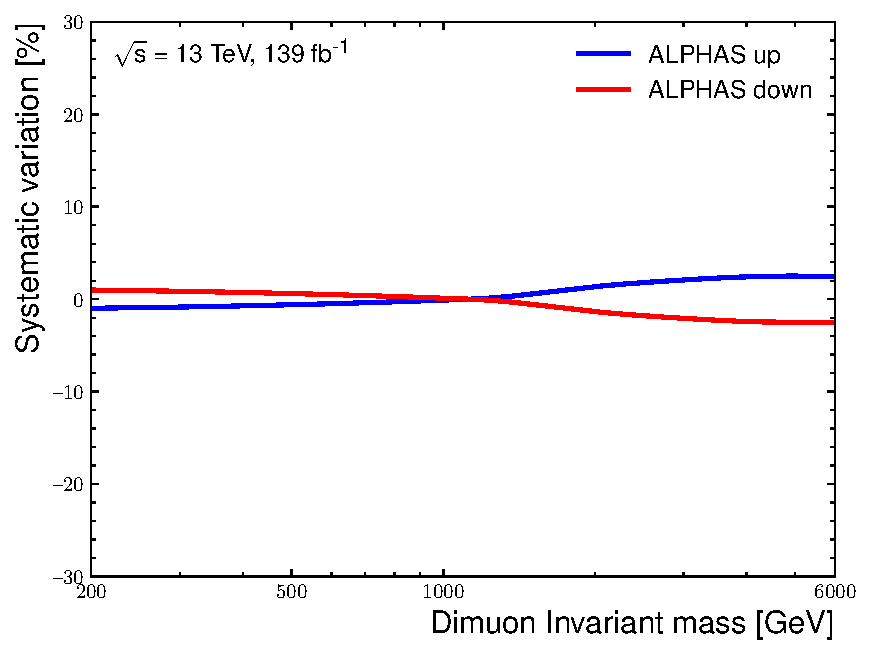
\includegraphics[width=\textwidth]{figures/analysis/datamc/Uncertainties/theory/mm/backgroundTemplate_KF_ALPHAS__1up.pdf}
        \caption{}
        \label{fig:uncert:mmalpha}
    \end{subfigure}
    \begin{subfigure}[h]{0.42\textwidth}
        \centering
        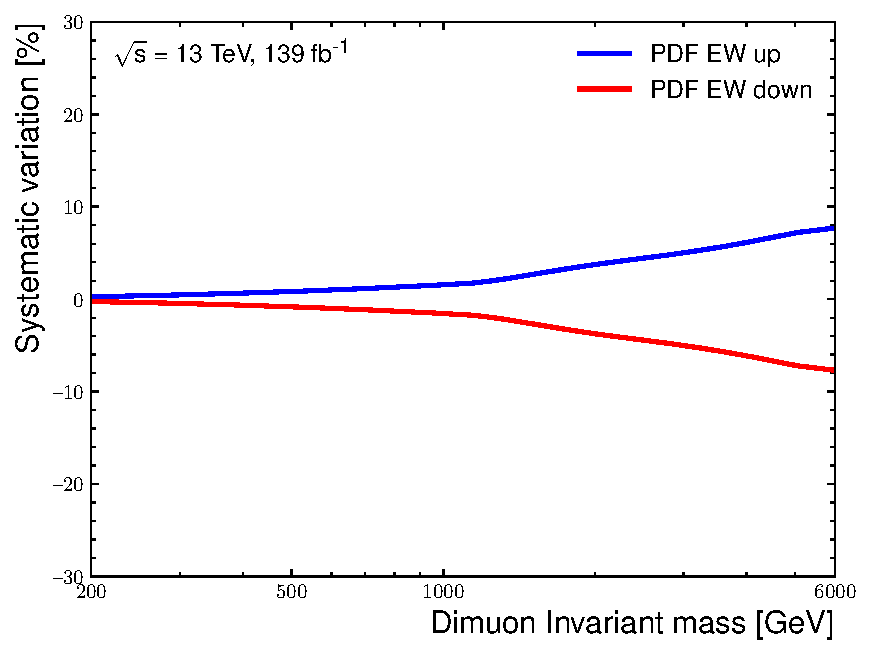
\includegraphics[width=\textwidth]{figures/analysis/datamc/Uncertainties/theory/mm/backgroundTemplate_KF_PDF_EW__1up.pdf}
        \caption{}
        \label{fig:uncert:mmEW}
    \end{subfigure}
    % \begin{subfigure}[h]{0.42\textwidth}
    %     \centering
    %     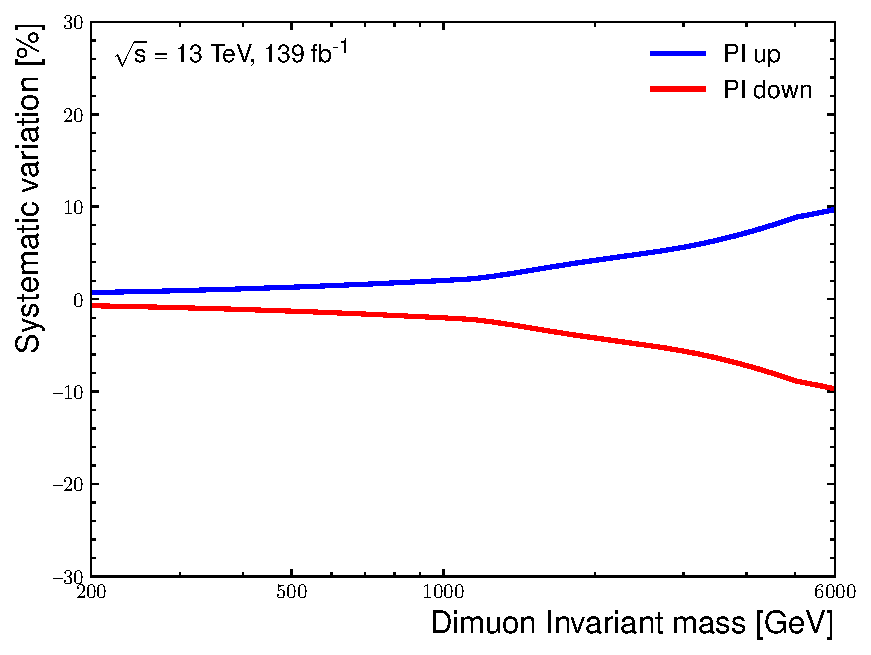
\includegraphics[width=\textwidth]{figures/analysis/datamc/Uncertainties/theory/mm/backgroundTemplate_KF_PI__1up.pdf}
    %     \label{fig:uncert:mmPI}
    % \end{subfigure}
    \begin{subfigure}[h]{0.42\textwidth}
        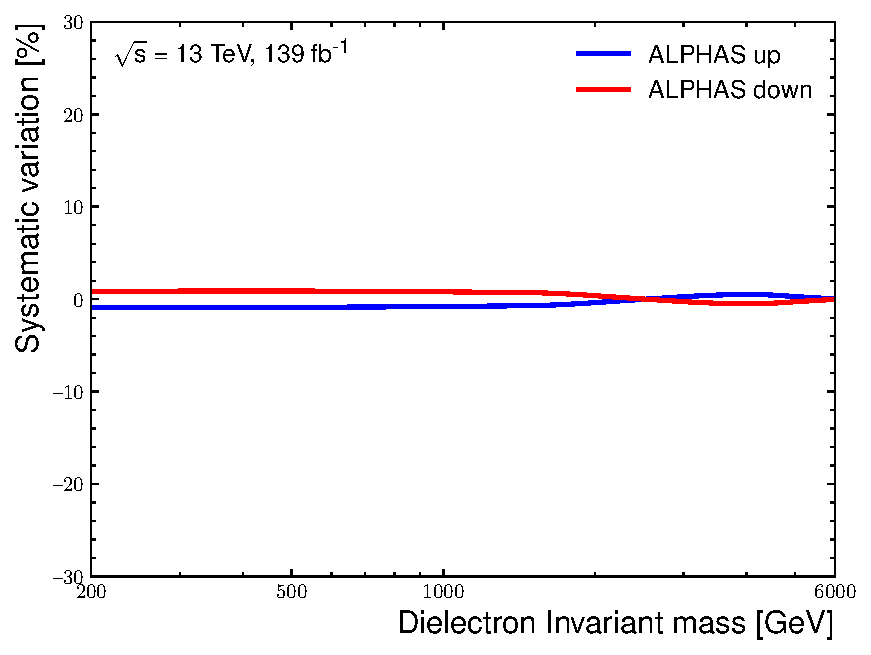
\includegraphics[width=\textwidth]{figures/analysis/datamc/Uncertainties/theory/ee/backgroundTemplate_KF_ALPHAS__1up.pdf}
        \caption{}
        \label{fig:uncert:eealpha}
    \end{subfigure}
    \begin{subfigure}[h]{0.42\textwidth}
        \centering
        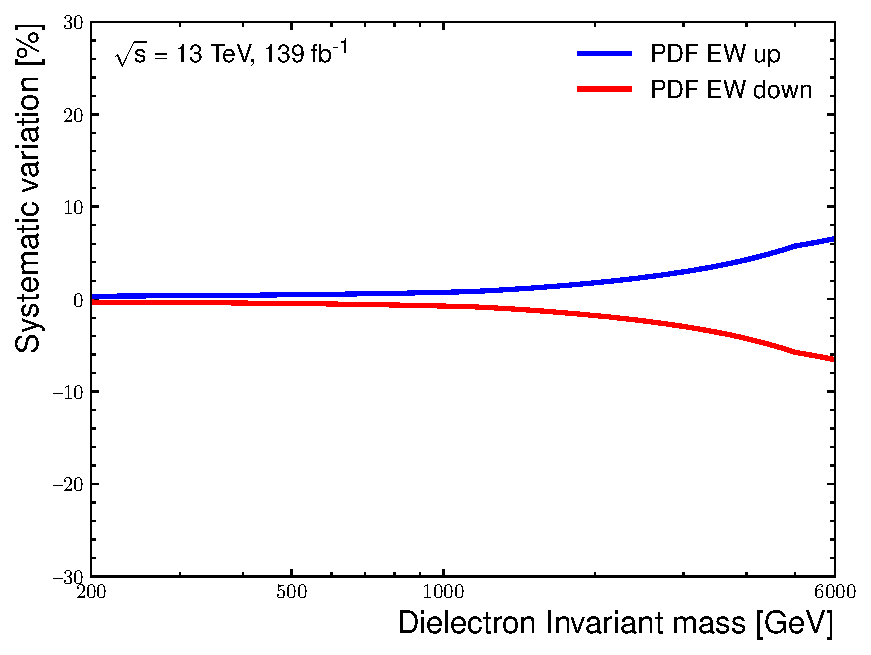
\includegraphics[width=\textwidth]{figures/analysis/datamc/Uncertainties/theory/ee/backgroundTemplate_KF_PDF_EW__1up.pdf}
        \caption{}
        \label{fig:uncert:eeEW}
    \end{subfigure}
    % \begin{subfigure}[h]{0.42\textwidth}
    %     \centering
    %     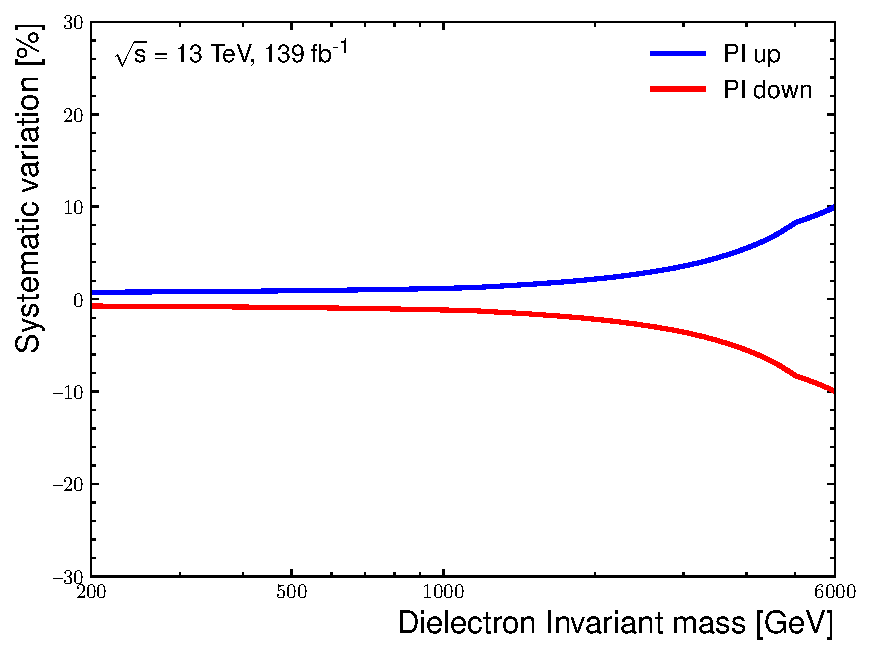
\includegraphics[width=\textwidth]{figures/analysis/datamc/Uncertainties/theory/ee/backgroundTemplate_KF_PI__1up.pdf}
    %     \label{fig:uncert:eePI}
    % \end{subfigure}
    \caption{Systematic uncertainties due to corrections applied to the CT10NNLO PDF. The uncertainty related to the strong coupling constant ($\alpha_s$) (a)/(b) and EW (c)/(d) corrections in the electron and muon channels, respectively.}
    \label{fig:uncert:theoryConstants}
\end{figure}

\subsubsection{Top-quark and diboson background uncertainty}
An uncertainty arises from the cross-section to which the top and diboson samples are normalised to. The normalisation uncertainty for the top background is estimated to be a 4\%~\cite{Czakon:2011xx}. The uncertainty on the diboson production cross-section is estimated to be between 5\% and 10\%~\cite{Butterworth:1287902}. A conservative normalisation uncertainty of 10\% is assigned to the diboson background. Since both uncertainties are normalisation uncertainties with a flat change of the invariant-mass distribution, the impact on the data-driven background estimate is expected to be negligible. 

\clearpage